\documentclass[1p]{elsarticle_modified}
%\bibliographystyle{elsarticle-num}

%\usepackage[colorlinks]{hyperref}
%\usepackage{abbrmath_seonhwa} %\Abb, \Ascr, \Acal ,\Abf, \Afrak
\usepackage{amsfonts}
\usepackage{amssymb}
\usepackage{amsmath}
\usepackage{amsthm}
\usepackage{scalefnt}
\usepackage{amsbsy}
\usepackage{kotex}
\usepackage{caption}
\usepackage{subfig}
\usepackage{color}
\usepackage{graphicx}
\usepackage{xcolor} %% white, black, red, green, blue, cyan, magenta, yellow
\usepackage{float}
\usepackage{setspace}
\usepackage{hyperref}

\usepackage{tikz}
\usetikzlibrary{arrows}

\usepackage{multirow}
\usepackage{array} % fixed length table
\usepackage{hhline}

%%%%%%%%%%%%%%%%%%%%%
\makeatletter
\renewcommand*\env@matrix[1][\arraystretch]{%
	\edef\arraystretch{#1}%
	\hskip -\arraycolsep
	\let\@ifnextchar\new@ifnextchar
	\array{*\c@MaxMatrixCols c}}
\makeatother %https://tex.stackexchange.com/questions/14071/how-can-i-increase-the-line-spacing-in-a-matrix
%%%%%%%%%%%%%%%

\usepackage[normalem]{ulem}

\newcommand{\msout}[1]{\ifmmode\text{\sout{\ensuremath{#1}}}\else\sout{#1}\fi}
%SOURCE: \msout is \stkout macro in https://tex.stackexchange.com/questions/20609/strikeout-in-math-mode

\newcommand{\cancel}[1]{
	\ifmmode
	{\color{red}\msout{#1}}
	\else
	{\color{red}\sout{#1}}
	\fi
}

\newcommand{\add}[1]{
	{\color{blue}\uwave{#1}}
}

\newcommand{\replace}[2]{
	\ifmmode
	{\color{red}\msout{#1}}{\color{blue}\uwave{#2}}
	\else
	{\color{red}\sout{#1}}{\color{blue}\uwave{#2}}
	\fi
}

\newcommand{\Sol}{\mathcal{S}} %segment
\newcommand{\D}{D} %diagram
\newcommand{\A}{\mathcal{A}} %arc


%%%%%%%%%%%%%%%%%%%%%%%%%%%%%5 test

\def\sl{\operatorname{\textup{SL}}(2,\Cbb)}
\def\psl{\operatorname{\textup{PSL}}(2,\Cbb)}
\def\quan{\mkern 1mu \triangleright \mkern 1mu}

\theoremstyle{definition}
\newtheorem{thm}{Theorem}[section]
\newtheorem{prop}[thm]{Proposition}
\newtheorem{lem}[thm]{Lemma}
\newtheorem{ques}[thm]{Question}
\newtheorem{cor}[thm]{Corollary}
\newtheorem{defn}[thm]{Definition}
\newtheorem{exam}[thm]{Example}
\newtheorem{rmk}[thm]{Remark}
\newtheorem{alg}[thm]{Algorithm}

\newcommand{\I}{\sqrt{-1}}
\begin{document}

%\begin{frontmatter}
%
%\title{Boundary parabolic representations of knots up to 8 crossings}
%
%%% Group authors per affiliation:
%\author{Yunhi Cho} 
%\address{Department of Mathematics, University of Seoul, Seoul, Korea}
%\ead{yhcho@uos.ac.kr}
%
%
%\author{Seonhwa Kim} %\fnref{s_kim}}
%\address{Center for Geometry and Physics, Institute for Basic Science, Pohang, 37673, Korea}
%\ead{ryeona17@ibs.re.kr}
%
%\author{Hyuk Kim}
%\address{Department of Mathematical Sciences, Seoul National University, Seoul 08826, Korea}
%\ead{hyukkim@snu.ac.kr}
%
%\author{Seokbeom Yoon}
%\address{Department of Mathematical Sciences, Seoul National University, Seoul, 08826,  Korea}
%\ead{sbyoon15@snu.ac.kr}
%
%\begin{abstract}
%We find all boundary parabolic representation of knots up to 8 crossings.
%
%\end{abstract}
%\begin{keyword}
%    \MSC[2010] 57M25 
%\end{keyword}
%
%\end{frontmatter}

%\linenumbers
%\tableofcontents
%
\newcommand\colored[1]{\textcolor{white}{\rule[-0.35ex]{0.8em}{1.4ex}}\kern-0.8em\color{red} #1}%
%\newcommand\colored[1]{\textcolor{white}{ #1}\kern-2.17ex	\textcolor{white}{ #1}\kern-1.81ex	\textcolor{white}{ #1}\kern-2.15ex\color{red}#1	}

{\Large $\underline{12a_{1040}~(K12a_{1040})}$}

\setlength{\tabcolsep}{10pt}
\renewcommand{\arraystretch}{1.6}
\vspace{1cm}\begin{tabular}{m{100pt}>{\centering\arraybackslash}m{274pt}}
\multirow{5}{120pt}{
	\centering
	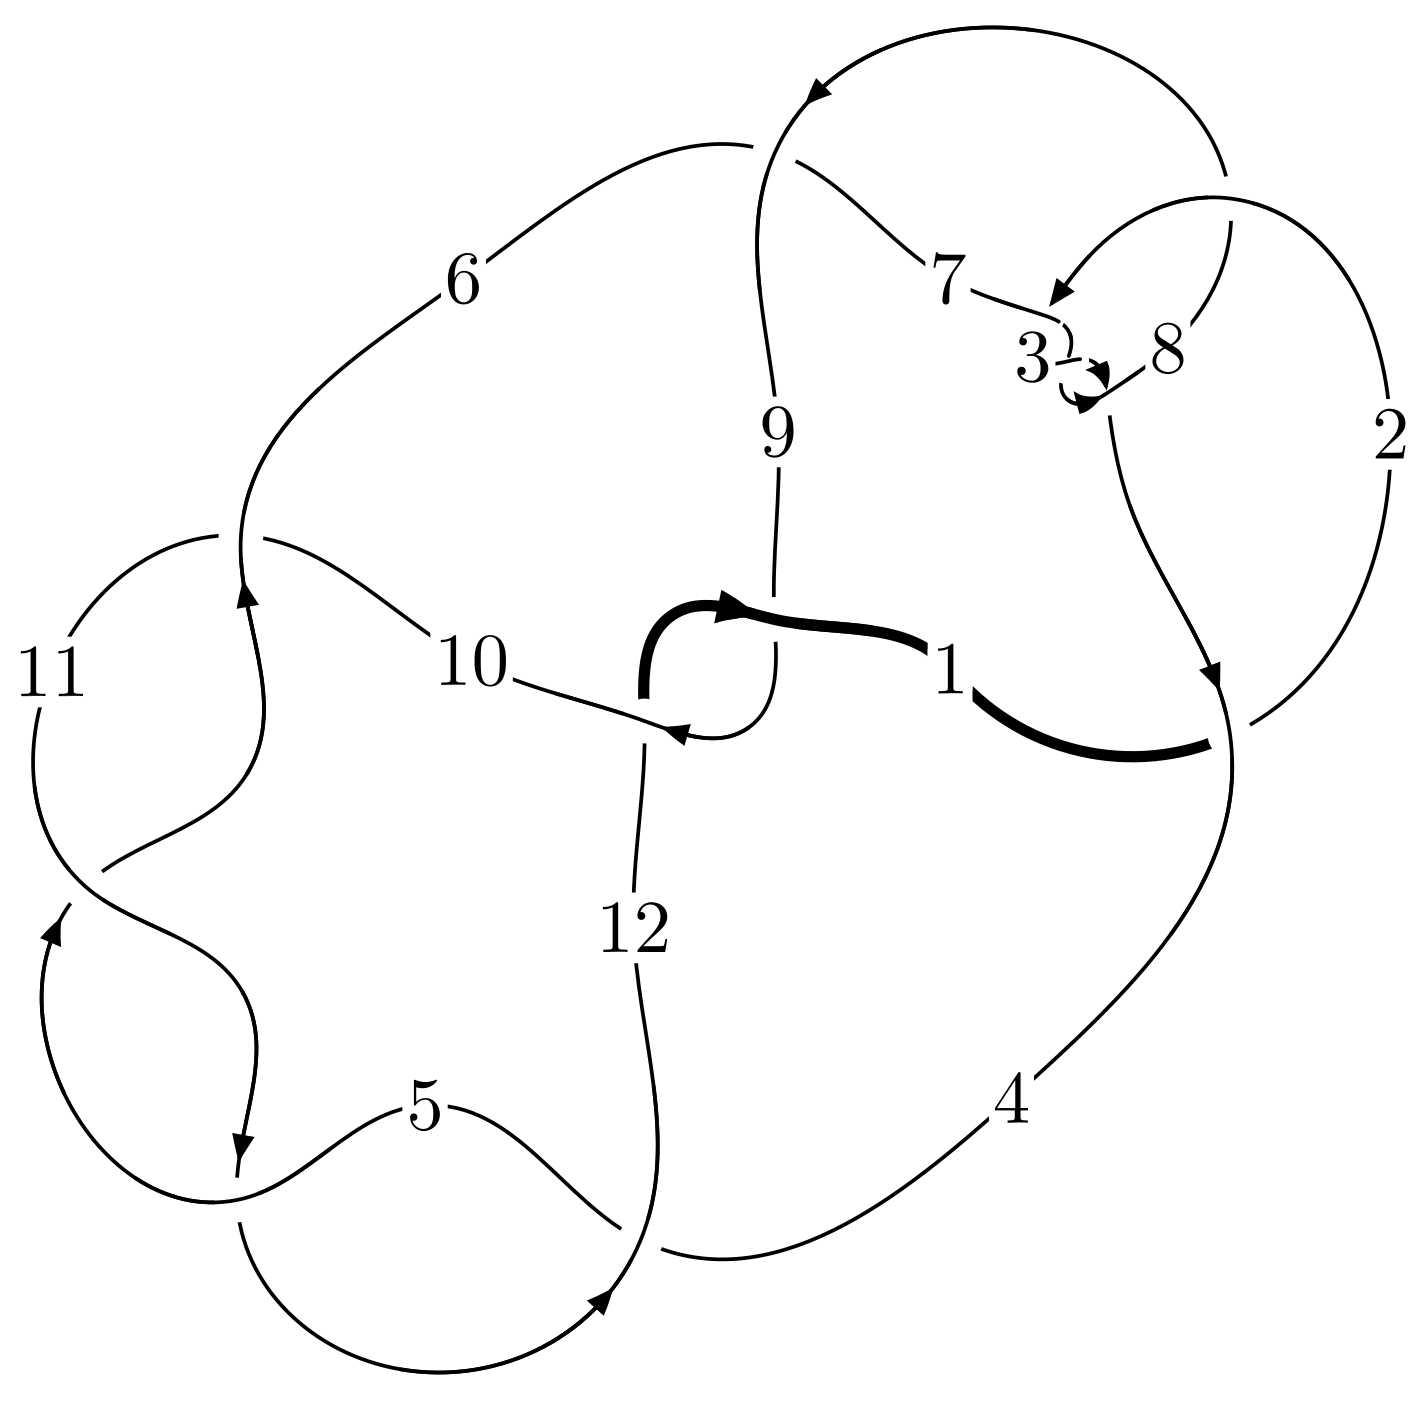
\includegraphics[width=112pt]{../../../GIT/diagram.site/Diagrams/png/1841_12a_1040.png}\\
\ \ \ A knot diagram\footnotemark}&
\allowdisplaybreaks
\textbf{Linearized knot diagam} \\
\cline{2-2}
 &
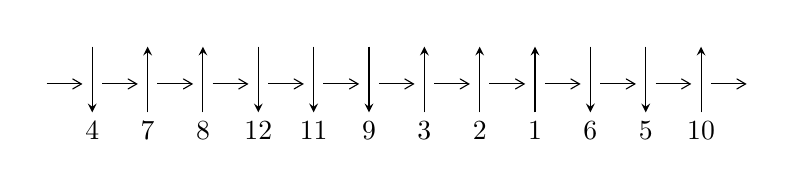
\begin{tikzpicture}[x=20pt, y=17pt]
	% nodes
	\node (C0) at (0, 0) {};
	\node (C1) at (1, 0) {};
	\node (C1U) at (1, +1) {};
	\node (C1D) at (1, -1) {4};

	\node (C2) at (2, 0) {};
	\node (C2U) at (2, +1) {};
	\node (C2D) at (2, -1) {7};

	\node (C3) at (3, 0) {};
	\node (C3U) at (3, +1) {};
	\node (C3D) at (3, -1) {8};

	\node (C4) at (4, 0) {};
	\node (C4U) at (4, +1) {};
	\node (C4D) at (4, -1) {12};

	\node (C5) at (5, 0) {};
	\node (C5U) at (5, +1) {};
	\node (C5D) at (5, -1) {11};

	\node (C6) at (6, 0) {};
	\node (C6U) at (6, +1) {};
	\node (C6D) at (6, -1) {9};

	\node (C7) at (7, 0) {};
	\node (C7U) at (7, +1) {};
	\node (C7D) at (7, -1) {3};

	\node (C8) at (8, 0) {};
	\node (C8U) at (8, +1) {};
	\node (C8D) at (8, -1) {2};

	\node (C9) at (9, 0) {};
	\node (C9U) at (9, +1) {};
	\node (C9D) at (9, -1) {1};

	\node (C10) at (10, 0) {};
	\node (C10U) at (10, +1) {};
	\node (C10D) at (10, -1) {6};

	\node (C11) at (11, 0) {};
	\node (C11U) at (11, +1) {};
	\node (C11D) at (11, -1) {5};

	\node (C12) at (12, 0) {};
	\node (C12U) at (12, +1) {};
	\node (C12D) at (12, -1) {10};
	\node (C13) at (13, 0) {};

	% arrows
	\draw[->,>={angle 60}]
	(C0) edge (C1) (C1) edge (C2) (C2) edge (C3) (C3) edge (C4) (C4) edge (C5) (C5) edge (C6) (C6) edge (C7) (C7) edge (C8) (C8) edge (C9) (C9) edge (C10) (C10) edge (C11) (C11) edge (C12) (C12) edge (C13) ;	\draw[->,>=stealth]
	(C1U) edge (C1D) (C2D) edge (C2U) (C3D) edge (C3U) (C4U) edge (C4D) (C5U) edge (C5D) (C6U) edge (C6D) (C7D) edge (C7U) (C8D) edge (C8U) (C9D) edge (C9U) (C10U) edge (C10D) (C11U) edge (C11D) (C12D) edge (C12U) ;
	\end{tikzpicture} \\
\hhline{~~} \\& 
\textbf{Solving Sequence} \\ \cline{2-2} 
 &
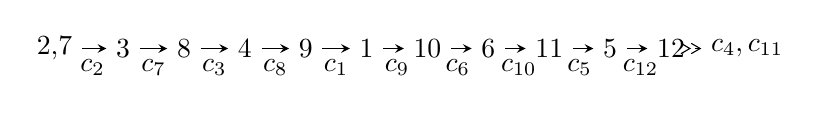
\begin{tikzpicture}[x=22pt, y=7pt]
	% node
	\node (A0) at (-1/8, 0) {2,7};
	\node (A1) at (1, 0) {3};
	\node (A2) at (2, 0) {8};
	\node (A3) at (3, 0) {4};
	\node (A4) at (4, 0) {9};
	\node (A5) at (5, 0) {1};
	\node (A6) at (6, 0) {10};
	\node (A7) at (7, 0) {6};
	\node (A8) at (8, 0) {11};
	\node (A9) at (9, 0) {5};
	\node (A10) at (10, 0) {12};
	\node (C1) at (1/2, -1) {$c_{2}$};
	\node (C2) at (3/2, -1) {$c_{7}$};
	\node (C3) at (5/2, -1) {$c_{3}$};
	\node (C4) at (7/2, -1) {$c_{8}$};
	\node (C5) at (9/2, -1) {$c_{1}$};
	\node (C6) at (11/2, -1) {$c_{9}$};
	\node (C7) at (13/2, -1) {$c_{6}$};
	\node (C8) at (15/2, -1) {$c_{10}$};
	\node (C9) at (17/2, -1) {$c_{5}$};
	\node (C10) at (19/2, -1) {$c_{12}$};
	\node (A11) at (45/4, 0) {$c_{4},c_{11}$};

	% edge
	\draw[->,>=stealth]	
	(A0) edge (A1) (A1) edge (A2) (A2) edge (A3) (A3) edge (A4) (A4) edge (A5) (A5) edge (A6) (A6) edge (A7) (A7) edge (A8) (A8) edge (A9) (A9) edge (A10) ;
	\draw[->>,>={angle 60}]	
	(A10) edge (A11);
\end{tikzpicture} \\ 

\end{tabular} \\

\footnotetext{
The image of knot diagram is generated by the software ``\textbf{Draw programme}" developed by Andrew Bartholomew(\url{http://www.layer8.co.uk/maths/draw/index.htm\#Running-draw}), where we modified some parts for our purpose(\url{https://github.com/CATsTAILs/LinksPainter}).
}\phantom \\ \newline 
\centering \textbf{Ideals for irreducible components\footnotemark of $X_{\text{par}}$} 
 
\begin{align*}
I^u_{1}&=\langle 
u^{57}- u^{56}+\cdots+u+1\rangle \\
\\
\end{align*}
\raggedright * 1 irreducible components of $\dim_{\mathbb{C}}=0$, with total 57 representations.\\
\footnotetext{All coefficients of polynomials are rational numbers. But the coefficients are sometimes approximated in decimal forms when there is not enough margin.}
\newpage
\renewcommand{\arraystretch}{1}
\centering \section*{I. $I^u_{1}= \langle u^{57}- u^{56}+\cdots+u+1 \rangle$}
\flushleft \textbf{(i) Arc colorings}\\
\begin{tabular}{m{7pt} m{180pt} m{7pt} m{180pt} }
\flushright $a_{2}=$&$\begin{pmatrix}1\\0\end{pmatrix}$ \\
\flushright $a_{7}=$&$\begin{pmatrix}0\\u\end{pmatrix}$ \\
\flushright $a_{3}=$&$\begin{pmatrix}1\\- u^2\end{pmatrix}$ \\
\flushright $a_{8}=$&$\begin{pmatrix}u\\- u^3+u\end{pmatrix}$ \\
\flushright $a_{4}=$&$\begin{pmatrix}- u^2+1\\u^4-2 u^2\end{pmatrix}$ \\
\flushright $a_{9}=$&$\begin{pmatrix}- u^3+2 u\\- u^3+u\end{pmatrix}$ \\
\flushright $a_{1}=$&$\begin{pmatrix}u^6-3 u^4+2 u^2+1\\- u^8+4 u^6-4 u^4\end{pmatrix}$ \\
\flushright $a_{10}=$&$\begin{pmatrix}- u^{17}+8 u^{15}-25 u^{13}+36 u^{11}-19 u^9-4 u^7+2 u^5+2 u^3+3 u\\u^{19}-9 u^{17}+32 u^{15}-55 u^{13}+43 u^{11}-9 u^9-4 u^5- u^3+u\end{pmatrix}$ \\
\flushright $a_{6}=$&$\begin{pmatrix}u^7-4 u^5+4 u^3\\u^7-3 u^5+2 u^3+u\end{pmatrix}$ \\
\flushright $a_{11}=$&$\begin{pmatrix}- u^{33}+16 u^{31}+\cdots+2 u^3+3 u\\- u^{33}+15 u^{31}+\cdots+2 u^3+u\end{pmatrix}$ \\
\flushright $a_{5}=$&$\begin{pmatrix}- u^{54}+25 u^{52}+\cdots+2 u^2+1\\u^{56}-26 u^{54}+\cdots+4 u^4-2 u^2\end{pmatrix}$ \\
\flushright $a_{12}=$&$\begin{pmatrix}u^{28}-13 u^{26}+\cdots+5 u^2+1\\- u^{30}+14 u^{28}+\cdots-4 u^4+u^2\end{pmatrix}$\\&\end{tabular}
\flushleft \textbf{(ii) Obstruction class $= -1$}\\~\\
\flushleft \textbf{(iii) Cusp Shapes $= -4 u^{55}+104 u^{53}+\cdots+20 u+2$}\\~\\
\newpage\renewcommand{\arraystretch}{1}
\flushleft \textbf{(iv) u-Polynomials at the component}\newline \\
\begin{tabular}{m{50pt}|m{274pt}}
Crossings & \hspace{64pt}u-Polynomials at each crossing \\
\hline $$\begin{aligned}c_{1},c_{6}\end{aligned}$$&$\begin{aligned}
&u^{57}-9 u^{56}+\cdots+417 u-41
\end{aligned}$\\
\hline $$\begin{aligned}c_{2},c_{3},c_{7}\end{aligned}$$&$\begin{aligned}
&u^{57}+u^{56}+\cdots+u-1
\end{aligned}$\\
\hline $$\begin{aligned}c_{4},c_{5},c_{10}\\c_{11}\end{aligned}$$&$\begin{aligned}
&u^{57}+u^{56}+\cdots- u-1
\end{aligned}$\\
\hline $$\begin{aligned}c_{8}\end{aligned}$$&$\begin{aligned}
&u^{57}-3 u^{56}+\cdots-313 u+175
\end{aligned}$\\
\hline $$\begin{aligned}c_{9},c_{12}\end{aligned}$$&$\begin{aligned}
&u^{57}+11 u^{56}+\cdots+57 u+11
\end{aligned}$\\
\hline
\end{tabular}\\~\\
\newpage\renewcommand{\arraystretch}{1}
\flushleft \textbf{(v) Riley Polynomials at the component}\newline \\
\begin{tabular}{m{50pt}|m{274pt}}
Crossings & \hspace{64pt}Riley Polynomials at each crossing \\
\hline $$\begin{aligned}c_{1},c_{6}\end{aligned}$$&$\begin{aligned}
&y^{57}+43 y^{56}+\cdots-48987 y-1681
\end{aligned}$\\
\hline $$\begin{aligned}c_{2},c_{3},c_{7}\end{aligned}$$&$\begin{aligned}
&y^{57}-53 y^{56}+\cdots-7 y-1
\end{aligned}$\\
\hline $$\begin{aligned}c_{4},c_{5},c_{10}\\c_{11}\end{aligned}$$&$\begin{aligned}
&y^{57}+63 y^{56}+\cdots-7 y-1
\end{aligned}$\\
\hline $$\begin{aligned}c_{8}\end{aligned}$$&$\begin{aligned}
&y^{57}-17 y^{56}+\cdots+297469 y-30625
\end{aligned}$\\
\hline $$\begin{aligned}c_{9},c_{12}\end{aligned}$$&$\begin{aligned}
&y^{57}+27 y^{56}+\cdots-3483 y-121
\end{aligned}$\\
\hline
\end{tabular}\\~\\
\newpage\flushleft \textbf{(vi) Complex Volumes and Cusp Shapes}
$$\begin{array}{c|c|c}  
\text{Solutions to }I^u_{1}& \I (\text{vol} + \sqrt{-1}CS) & \text{Cusp shape}\\
 \hline 
\begin{aligned}
u &= \phantom{-}1.167470 + 0.169882 I\end{aligned}
 & \phantom{-}5.94879 - 1.26768 I & \phantom{-0.000000 } 0 \\ \hline\begin{aligned}
u &= \phantom{-}1.167470 - 0.169882 I\end{aligned}
 & \phantom{-}5.94879 + 1.26768 I & \phantom{-0.000000 } 0 \\ \hline\begin{aligned}
u &= -0.380989 + 0.687075 I\end{aligned}
 & \phantom{-}7.59135 - 9.78879 I & \phantom{-}4.20807 + 7.63690 I \\ \hline\begin{aligned}
u &= -0.380989 - 0.687075 I\end{aligned}
 & \phantom{-}7.59135 + 9.78879 I & \phantom{-}4.20807 - 7.63690 I \\ \hline\begin{aligned}
u &= -1.210720 + 0.186692 I\end{aligned}
 & -0.388499 - 1.147720 I & \phantom{-0.000000 } 0 \\ \hline\begin{aligned}
u &= -1.210720 - 0.186692 I\end{aligned}
 & -0.388499 + 1.147720 I & \phantom{-0.000000 } 0 \\ \hline\begin{aligned}
u &= -0.450772 + 0.625585 I\end{aligned}
 & \phantom{-}12.14170 - 2.06019 I & \phantom{-}8.03202 + 3.36390 I \\ \hline\begin{aligned}
u &= -0.450772 - 0.625585 I\end{aligned}
 & \phantom{-}12.14170 + 2.06019 I & \phantom{-}8.03202 - 3.36390 I \\ \hline\begin{aligned}
u &= \phantom{-}0.370067 + 0.674356 I\end{aligned}
 & \phantom{-}0.31418 + 7.17616 I & \phantom{-}0.93396 - 9.10668 I \\ \hline\begin{aligned}
u &= \phantom{-}0.370067 - 0.674356 I\end{aligned}
 & \phantom{-}0.31418 - 7.17616 I & \phantom{-}0.93396 + 9.10668 I \\ \hline\begin{aligned}
u &= -0.535939 + 0.537357 I\end{aligned}
 & \phantom{-}8.22131 + 5.67967 I & \phantom{-}5.83026 - 1.65476 I \\ \hline\begin{aligned}
u &= -0.535939 - 0.537357 I\end{aligned}
 & \phantom{-}8.22131 - 5.67967 I & \phantom{-}5.83026 + 1.65476 I \\ \hline\begin{aligned}
u &= \phantom{-}1.236620 + 0.206975 I\end{aligned}
 & -0.13889 + 5.01254 I & \phantom{-0.000000 } 0 \\ \hline\begin{aligned}
u &= \phantom{-}1.236620 - 0.206975 I\end{aligned}
 & -0.13889 - 5.01254 I & \phantom{-0.000000 } 0 \\ \hline\begin{aligned}
u &= -0.355064 + 0.654949 I\end{aligned}
 & -0.47604 - 3.30732 I & -1.43106 + 3.04352 I \\ \hline\begin{aligned}
u &= -0.355064 - 0.654949 I\end{aligned}
 & -0.47604 + 3.30732 I & -1.43106 - 3.04352 I \\ \hline\begin{aligned}
u &= \phantom{-}0.418277 + 0.595875 I\end{aligned}
 & \phantom{-}3.97873 + 1.92695 I & \phantom{-}7.08631 - 3.98477 I \\ \hline\begin{aligned}
u &= \phantom{-}0.418277 - 0.595875 I\end{aligned}
 & \phantom{-}3.97873 - 1.92695 I & \phantom{-}7.08631 + 3.98477 I \\ \hline\begin{aligned}
u &= \phantom{-}0.514622 + 0.512995 I\end{aligned}
 & \phantom{-}0.95022 - 3.20263 I & \phantom{-}2.71277 + 3.09003 I \\ \hline\begin{aligned}
u &= \phantom{-}0.514622 - 0.512995 I\end{aligned}
 & \phantom{-}0.95022 + 3.20263 I & \phantom{-}2.71277 - 3.09003 I \\ \hline\begin{aligned}
u &= -1.255720 + 0.225833 I\end{aligned}
 & \phantom{-}6.68945 - 7.58268 I & \phantom{-0.000000 } 0 \\ \hline\begin{aligned}
u &= -1.255720 - 0.225833 I\end{aligned}
 & \phantom{-}6.68945 + 7.58268 I & \phantom{-0.000000 } 0 \\ \hline\begin{aligned}
u &= -1.27874\phantom{ +0.000000I}\end{aligned}
 & \phantom{-}2.94486\phantom{ +0.000000I} & \phantom{-0.000000 } 0 \\ \hline\begin{aligned}
u &= \phantom{-}0.301202 + 0.630196 I\end{aligned}
 & \phantom{-}5.12502 + 1.19979 I & \phantom{-}1.84526 - 3.54784 I \\ \hline\begin{aligned}
u &= \phantom{-}0.301202 - 0.630196 I\end{aligned}
 & \phantom{-}5.12502 - 1.19979 I & \phantom{-}1.84526 + 3.54784 I \\ \hline\begin{aligned}
u &= -0.464588 + 0.473428 I\end{aligned}
 & \phantom{-}0.149387 - 0.437986 I & \phantom{-}0.20836 + 3.87750 I \\ \hline\begin{aligned}
u &= -0.464588 - 0.473428 I\end{aligned}
 & \phantom{-}0.149387 + 0.437986 I & \phantom{-}0.20836 - 3.87750 I \\ \hline\begin{aligned}
u &= \phantom{-}1.336280 + 0.067950 I\end{aligned}
 & \phantom{-}4.76158 + 2.12463 I & \phantom{-0.000000 } 0 \\ \hline\begin{aligned}
u &= \phantom{-}1.336280 - 0.067950 I\end{aligned}
 & \phantom{-}4.76158 - 2.12463 I & \phantom{-0.000000 } 0 \\ \hline\begin{aligned}
u &= \phantom{-}0.053954 + 0.654719 I\end{aligned}
 & \phantom{-}2.66786 + 4.37051 I & -1.69929 - 3.89268 I\\
 \hline 
 \end{array}$$\newpage$$\begin{array}{c|c|c}  
\text{Solutions to }I^u_{1}& \I (\text{vol} + \sqrt{-1}CS) & \text{Cusp shape}\\
 \hline 
\begin{aligned}
u &= \phantom{-}0.053954 - 0.654719 I\end{aligned}
 & \phantom{-}2.66786 - 4.37051 I & -1.69929 + 3.89268 I \\ \hline\begin{aligned}
u &= -0.019054 + 0.641634 I\end{aligned}
 & -3.95983 - 1.90551 I & -5.97209 + 4.06985 I \\ \hline\begin{aligned}
u &= -0.019054 - 0.641634 I\end{aligned}
 & -3.95983 + 1.90551 I & -5.97209 - 4.06985 I \\ \hline\begin{aligned}
u &= -1.395500 + 0.073443 I\end{aligned}
 & \phantom{-}12.03160 - 3.33838 I & \phantom{-0.000000 } 0 \\ \hline\begin{aligned}
u &= -1.395500 - 0.073443 I\end{aligned}
 & \phantom{-}12.03160 + 3.33838 I & \phantom{-0.000000 } 0 \\ \hline\begin{aligned}
u &= \phantom{-}0.521676 + 0.299528 I\end{aligned}
 & \phantom{-}6.18669 + 2.12511 I & \phantom{-}5.30374 - 3.18757 I \\ \hline\begin{aligned}
u &= \phantom{-}0.521676 - 0.299528 I\end{aligned}
 & \phantom{-}6.18669 - 2.12511 I & \phantom{-}5.30374 + 3.18757 I \\ \hline\begin{aligned}
u &= -1.42263 + 0.23603 I\end{aligned}
 & \phantom{-}10.65770 - 4.35539 I & \phantom{-0.000000 } 0 \\ \hline\begin{aligned}
u &= -1.42263 - 0.23603 I\end{aligned}
 & \phantom{-}10.65770 + 4.35539 I & \phantom{-0.000000 } 0 \\ \hline\begin{aligned}
u &= \phantom{-}1.44389 + 0.19016 I\end{aligned}
 & \phantom{-}6.16952 + 2.93600 I & \phantom{-0.000000 } 0 \\ \hline\begin{aligned}
u &= \phantom{-}1.44389 - 0.19016 I\end{aligned}
 & \phantom{-}6.16952 - 2.93600 I & \phantom{-0.000000 } 0 \\ \hline\begin{aligned}
u &= \phantom{-}1.44231 + 0.24847 I\end{aligned}
 & \phantom{-}5.29940 + 6.61308 I & \phantom{-0.000000 } 0 \\ \hline\begin{aligned}
u &= \phantom{-}1.44231 - 0.24847 I\end{aligned}
 & \phantom{-}5.29940 - 6.61308 I & \phantom{-0.000000 } 0 \\ \hline\begin{aligned}
u &= -1.45405 + 0.22055 I\end{aligned}
 & \phantom{-}9.99378 - 4.92353 I & \phantom{-0.000000 } 0 \\ \hline\begin{aligned}
u &= -1.45405 - 0.22055 I\end{aligned}
 & \phantom{-}9.99378 + 4.92353 I & \phantom{-0.000000 } 0 \\ \hline\begin{aligned}
u &= -1.46020 + 0.18074 I\end{aligned}
 & \phantom{-}7.24551 + 0.69473 I & \phantom{-0.000000 } 0 \\ \hline\begin{aligned}
u &= -1.46020 - 0.18074 I\end{aligned}
 & \phantom{-}7.24551 - 0.69473 I & \phantom{-0.000000 } 0 \\ \hline\begin{aligned}
u &= -1.44938 + 0.25463 I\end{aligned}
 & \phantom{-}6.16341 - 10.57050 I & \phantom{-0.000000 } 0 \\ \hline\begin{aligned}
u &= -1.44938 - 0.25463 I\end{aligned}
 & \phantom{-}6.16341 + 10.57050 I & \phantom{-0.000000 } 0 \\ \hline\begin{aligned}
u &= \phantom{-}1.45510 + 0.25844 I\end{aligned}
 & \phantom{-}13.4982 + 13.2410 I & \phantom{-0.000000 } 0 \\ \hline\begin{aligned}
u &= \phantom{-}1.45510 - 0.25844 I\end{aligned}
 & \phantom{-}13.4982 - 13.2410 I & \phantom{-0.000000 } 0 \\ \hline\begin{aligned}
u &= \phantom{-}1.47223 + 0.17915 I\end{aligned}
 & \phantom{-}14.6669 - 3.1156 I & \phantom{-0.000000 } 0 \\ \hline\begin{aligned}
u &= \phantom{-}1.47223 - 0.17915 I\end{aligned}
 & \phantom{-}14.6669 + 3.1156 I & \phantom{-0.000000 } 0 \\ \hline\begin{aligned}
u &= \phantom{-}1.46992 + 0.22438 I\end{aligned}
 & \phantom{-}18.3360 + 5.1622 I & \phantom{-0.000000 } 0 \\ \hline\begin{aligned}
u &= \phantom{-}1.46992 - 0.22438 I\end{aligned}
 & \phantom{-}18.3360 - 5.1622 I & \phantom{-0.000000 } 0 \\ \hline\begin{aligned}
u &= -0.209648 + 0.330630 I\end{aligned}
 & \phantom{-}0.018322 - 0.795288 I & \phantom{-}0.54519 + 8.56502 I \\ \hline\begin{aligned}
u &= -0.209648 - 0.330630 I\end{aligned}
 & \phantom{-}0.018322 + 0.795288 I & \phantom{-}0.54519 - 8.56502 I\\
 \hline 
 \end{array}$$\newpage
\newpage\renewcommand{\arraystretch}{1}
\centering \section*{ II. u-Polynomials}
\begin{tabular}{m{50pt}|m{274pt}}
Crossings & \hspace{64pt}u-Polynomials at each crossing \\
\hline $$\begin{aligned}c_{1},c_{6}\end{aligned}$$&$\begin{aligned}
&u^{57}-9 u^{56}+\cdots+417 u-41
\end{aligned}$\\
\hline $$\begin{aligned}c_{2},c_{3},c_{7}\end{aligned}$$&$\begin{aligned}
&u^{57}+u^{56}+\cdots+u-1
\end{aligned}$\\
\hline $$\begin{aligned}c_{4},c_{5},c_{10}\\c_{11}\end{aligned}$$&$\begin{aligned}
&u^{57}+u^{56}+\cdots- u-1
\end{aligned}$\\
\hline $$\begin{aligned}c_{8}\end{aligned}$$&$\begin{aligned}
&u^{57}-3 u^{56}+\cdots-313 u+175
\end{aligned}$\\
\hline $$\begin{aligned}c_{9},c_{12}\end{aligned}$$&$\begin{aligned}
&u^{57}+11 u^{56}+\cdots+57 u+11
\end{aligned}$\\
\hline
\end{tabular}\newpage\renewcommand{\arraystretch}{1}
\centering \section*{ III. Riley Polynomials}
\begin{tabular}{m{50pt}|m{274pt}}
Crossings & \hspace{64pt}Riley Polynomials at each crossing \\
\hline $$\begin{aligned}c_{1},c_{6}\end{aligned}$$&$\begin{aligned}
&y^{57}+43 y^{56}+\cdots-48987 y-1681
\end{aligned}$\\
\hline $$\begin{aligned}c_{2},c_{3},c_{7}\end{aligned}$$&$\begin{aligned}
&y^{57}-53 y^{56}+\cdots-7 y-1
\end{aligned}$\\
\hline $$\begin{aligned}c_{4},c_{5},c_{10}\\c_{11}\end{aligned}$$&$\begin{aligned}
&y^{57}+63 y^{56}+\cdots-7 y-1
\end{aligned}$\\
\hline $$\begin{aligned}c_{8}\end{aligned}$$&$\begin{aligned}
&y^{57}-17 y^{56}+\cdots+297469 y-30625
\end{aligned}$\\
\hline $$\begin{aligned}c_{9},c_{12}\end{aligned}$$&$\begin{aligned}
&y^{57}+27 y^{56}+\cdots-3483 y-121
\end{aligned}$\\
\hline
\end{tabular}
\vskip 2pc
\end{document}